\documentclass[12pt]{article}
\usepackage[margin=1.5cm]{geometry}
\usepackage{parskip}
\usepackage{amsmath}
\usepackage{amssymb}
\usepackage{amsfonts}
\usepackage{enumitem}
\usepackage{graphicx}
\usepackage{stmaryrd}
\graphicspath{ {./images/} }


\begin{document}
\begin{enumerate}[label=(\alph*)]

  \item
    The phase order problem is the problem of deciding in which order we should perform compiler transformations in order to obtain the best optimised code.

    \item
      From such a basic block, we generate a node for each instruction.

      Then, we add an edge from node $n_1$ to node $n_2$ if the instruction for $n_1$ occurs before the instruction for $n_2$ in the original program order, and there is a dependency between $n_1$ and $n_2$, i.e.:

      \begin{itemize}
            \item
              $n_1$ reads from a register that $n_2$ writes to
      \end{itemize}

      (we omit RAW hazards since we are in SSA form).

      \item
        A register inference graph can be obtained by performing live variable analysis.

        LVA involves running an algorithm like the following:

\begin{verbatim}
live[1..n] = {}
while (live[] changes)
  for i in 1..n do
    live[i] = big_union(s in succ(i), live[s]) \ kill(i) U gen(i)
\end{verbatim}

Where $kill(i)$ returns the variables defined by instruction $i$ and $gen(i)$ returns the variables referenced by instruction $i$.

Then, given live sets for each instruction, we create a graph containing a node for every variable, and add an edge between two nodes if there exists a live variable set which they are both in.

For colouring this graph with registers, we require that at least one of the variables has fewer clashes than we have registers, or else we have to spill to memory.

\item
  In the first program, we get the two variants (LVA sets annotated)

\begin{verbatim}
add   t1, a, b   {a, b, c}
add#2 t2, c      {t1, c}
add#3 t3, c      {t1, t2, c}
mul   t4, t2, t3 {t1, t2, t3}
sub   z,  t1, t4 {t1, t4}

add#2 t2, c      {a, b, c}
add#3 t3, c      {t2, a, b, c}
mul   t4, t2, t3 {t2, t3, a, b}
add   t1, a, b   {t4, a, b}
sub   z,  t1, t4 {t1, t4}
\end{verbatim}

This yields the following clash graphs:

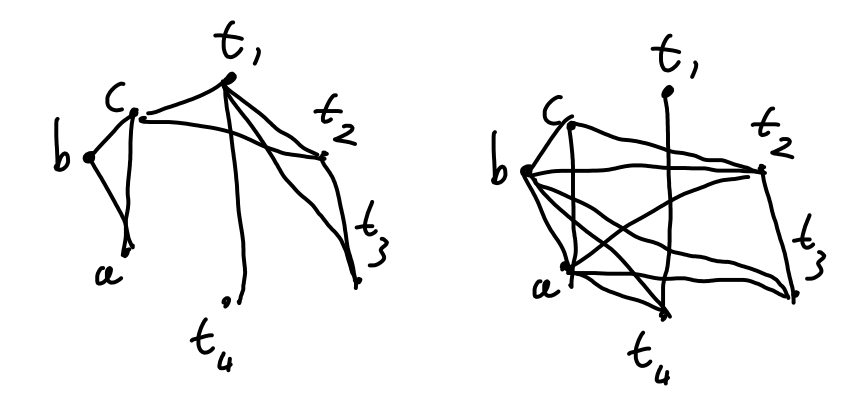
\includegraphics[scale=0.3]{clashgraph1}

We see that the first clash graph requires just 3 registers to colour, whereas the second clash graph requires 4 registers to colour (since there is an LVA set of size 4)

In the second program, we get the two variants (LVA sets annotated):

\begin{verbatim}
add t1,a,b   {a, b, c}
add#2 t2,c   {t1, a, b, c}
add#3 t3,c   {t1, t2, a, b, c}
mul t4,t2,t3 {t1, t2, t3, a, b}
sub t5,t1,t4 {t1, t4, a, b}
xor t6,t5,a  {t5, a, b}
xor z,t6,b   {t6, b}
    
add#2 t2,c   {a, b, c}
add#3 t3,c   {t2, a, b, c}
mul t4,t2,t3 {t2, t3, a, b}
add t1,a,b   {t4, a, b}
sub t5,t1,t4 {t1, t4, a, b}
xor t6,t5,a  {t5, a, b}
xor z,t6,b   {t6, b}
\end{verbatim}

And the following clash graphs:

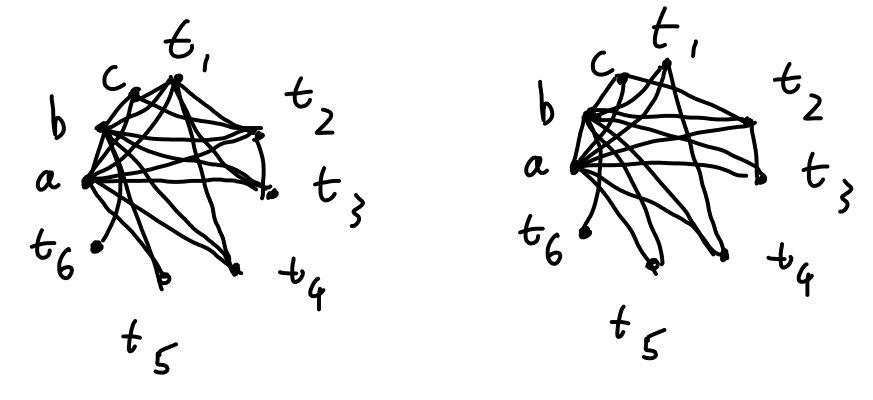
\includegraphics[scale=0.3]{clashgraph2}
 
We see that the first clash graph requires at least 5 registers to colour, whereas the second clash graph requires only 4 registers to colour.

So, we see that there is no overall choice as to whether we should schedule instruction as late/early as possible for optimising register allocation, instead it depends on the program itself. In particular, we see that the first program performs better by scheduling the instruction as early as possible because its operands are dead after its definition, whereas the second program performs better by scheduling the instruction as late as possible because its operands are live after its definition (and the instruction has two unique operands that are different to its destination).



        
    \end{enumerate}
\end{document}
